\documentclass[tikz,border=5pt]{standalone}
\begin{document}

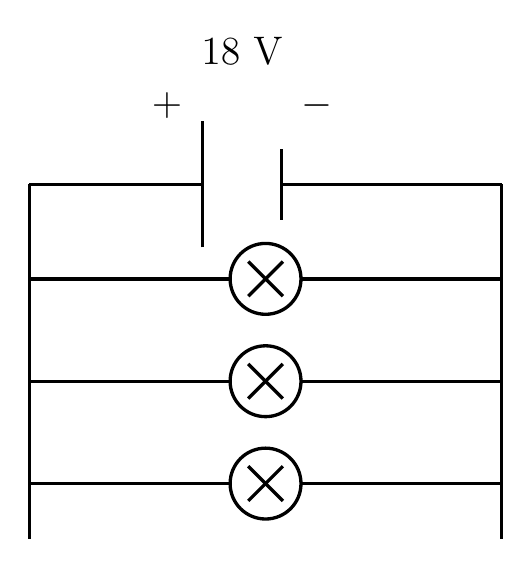
\begin{tikzpicture}[line width=1.2pt]

    % --- Dimensions principales ---
    \def\xleft{0}
    \def\xright{6}
    \def\ytop{5}
    \def\yA{3.8}
    \def\yB{2.5}
    \def\yC{1.2}
    \def\rlamp{0.45}

    % positions des ampoules
    \def\xlamp{3}

    % positions de la pile
    \def\xbatA{2.2}   % grande plaque
    \def\xbatB{3.2}   % petite plaque

    % -----------------------------
    % Rails verticaux
    % -----------------------------
    \draw (\xleft,\ytop) -- (\xleft,0.5);
    \draw (\xright,\ytop) -- (\xright,0.5);

    % -----------------------------
    % Fil du haut + pile
    % -----------------------------
    \draw (\xleft,\ytop) -- (\xbatA,\ytop);
    \draw (\xbatB,\ytop) -- (\xright,\ytop);

    % pile
    \draw (\xbatA,\ytop-0.8) -- (\xbatA,\ytop+0.8); % grande plaque
    \draw (\xbatB,\ytop-0.45) -- (\xbatB,\ytop+0.45); % petite plaque

    % signes + et -
    \node[font=\Large] at (\xbatA-0.45,\ytop+1.0) {$+$};
    \node[font=\Large] at (\xbatB+0.45,\ytop+1.0) {$-$};

    % texte tension
    \node[font=\Large] at ({(\xbatA+\xbatB)/2},\ytop+1.7) {18 V};

    % -----------------------------
    % Commande pour dessiner une ampoule
    % -----------------------------
    \newcommand{\Lampe}[2]{
        \draw (#1,#2) circle (\rlamp);
        \draw (#1-0.22,#2-0.22) -- (#1+0.22,#2+0.22);
        \draw (#1-0.22,#2+0.22) -- (#1+0.22,#2-0.22);
    }

    % -----------------------------
    % Branche 1
    % -----------------------------
    \draw (\xleft,\yA) -- (\xlamp-\rlamp,\yA);
    \draw (\xlamp+\rlamp,\yA) -- (\xright,\yA);
    \Lampe{\xlamp}{\yA}

    % -----------------------------
    % Branche 2
    % -----------------------------
    \draw (\xleft,\yB) -- (\xlamp-\rlamp,\yB);
    \draw (\xlamp+\rlamp,\yB) -- (\xright,\yB);
    \Lampe{\xlamp}{\yB}

    % -----------------------------
    % Branche 3
    % -----------------------------
    \draw (\xleft,\yC) -- (\xlamp-\rlamp,\yC);
    \draw (\xlamp+\rlamp,\yC) -- (\xright,\yC);
    \Lampe{\xlamp}{\yC}

\end{tikzpicture}

\end{document}